\documentclass[10pt, oneside]{article}

\usepackage[a4paper, total={5.5in, 9in}]{geometry}
\usepackage[ngerman]{babel}
\usepackage{import}

\import{../../.texit/include}{preamble}

\title{Einführung in die Künstliche Intelligenz\\[15pt]\Large{Übungsblatt 3}\\[10pt]\Large{SoSe 2025}}
\author{Volodymyr But\\[10pt]Hochschule Trier}
\date{}

% - - - - - - - - - - - - - - - - - - - - - - - - - - - - - - - - - - - - - - %

\begin{document}

\maketitle
\vspace{25px}

\setcounter{section}
{1} % 2
\section{Entscheidungsbaum erstellen}

\begin{enumerate}[(a)]
    \item Bestimmen Sie das beste Attribut für die Wurzel des Entscheidungsbaums.
        \begin{equation*}
            \text{Entropy}(S) = -\left(\dfrac{9}{14} \cdot \log_2 \dfrac{9}{14} + \left(1 - \dfrac{9}{14}\right) \cdot \log_2\left(1 - \dfrac{9}{14}\right)\right) \approx 0.94
        \end{equation*}
        \begin{enumerate}[1.]
           \item Attribut \verb|Outlook|
            \begin{gather*}
                \text{Entropy}(S_\text{Sunny}) \approx 0.97 \ \ \ \ \ \text{Entropy}(S_\text{Overcast}) = 0 \ \ \ \ \ \text{Entropy}(S_\text{Rain}) \approx 0.97 \\[5pt]
                \text{Gain}(S, \text{Outlook}) = 0.94 - 2 \cdot \dfrac{5}{14} \cdot 0.97 \approx 0.25
            \end{gather*}

           \item Attribut \verb|Humidity|
            \begin{gather*}
                \text{Entropy}(S_\text{High}) \approx 0.98 \ \ \ \ \ \ \text{Entropy}(S_\text{Normal}) \approx 0.59 \\[10pt]
                \text{Gain}(S, \text{Humidity}) = 0.94 - \left(\dfrac{7}{14} \cdot 0.98 + \dfrac{7}{14} \cdot 0.59\right) = 0.155
            \end{gather*}
           \item Attribut \verb|Wind|
            \begin{gather*}
                \text{Entropy}(S_\text{Weak}) \approx 0.81 \ \ \ \ \ \text{Entropy}(S_\text{Strong}) = 1 \\[10pt]
                \text{Gain}(S, \text{Wind}) = 0.94 - \left(\dfrac{8}{14} \cdot 0.81 + \dfrac{6}{14} \cdot 1\right) \approx 0.05
            \end{gather*}
    \end{enumerate}

    Das Attribut mit dem h"ochstens Information Gain ist Attribut
    \verb|Outlook|. Daher ist es auch das beste Attribut.

    \item Konstruieren Sie schrittweise einen Entscheidungsbaum für die obigen Trainingsdaten.

        Siehe Abbildung~\ref{fig:02-b}

    \item Wir möchten einen Datensatz zur Beispielmenge hinzufügen, so dass im
        Entscheidungsbaum zur erweiterten Trainingsmenge ein anderes Attribut
        an der Wurzel steht. Welchen Datensatz fügen Sie hinzu?

        Wir können den \verb|Outlook|-Wert unklarer machen, z.B. indem wir ein
        Beispiel mit \verb|Outlook = Overcast| und \verb|PlayTennis = No|
        hinzufügen. Dadurch ist \verb|Overcast| nicht mehr eindeutig mit
        \verb|Yes| verbunden, was den Information Gain von „Outlook“ reduziert.
        Dies kann dazu f"uhren, dass z.B \verb|Humidity| zur neuen Wurzel wird.

\end{enumerate}

\begin{figure}[p]
    \centering
    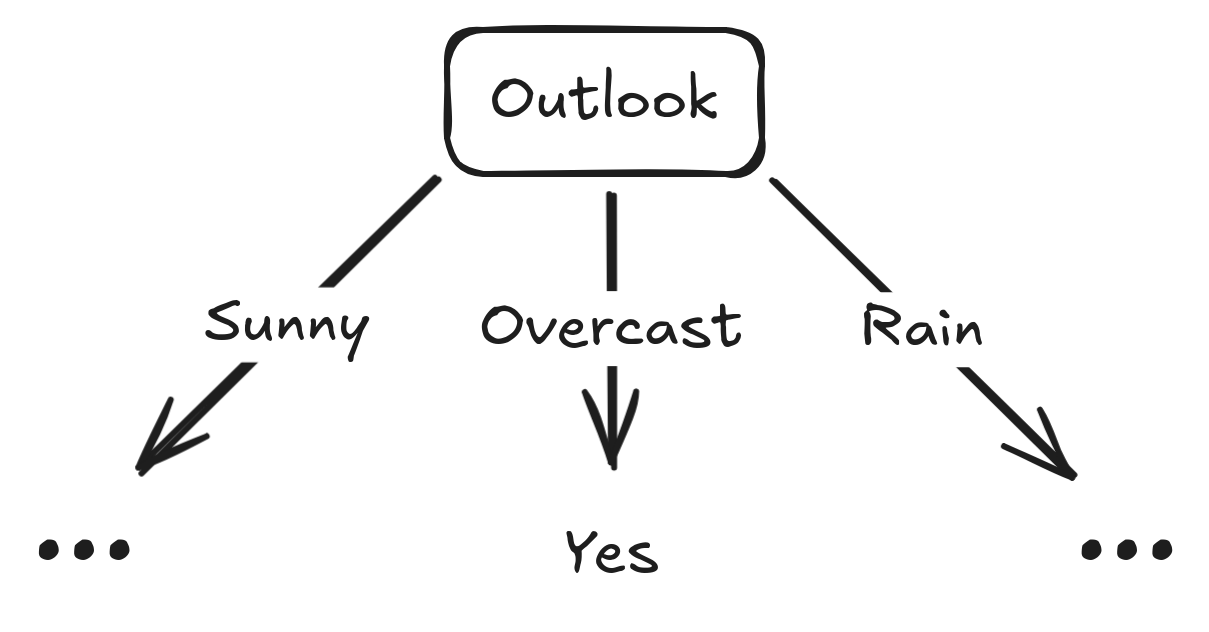
\includegraphics[width=1\textwidth]{./assets/02-b.png}
    \caption{}
    \label{fig:02-b}
\end{figure}

\FloatBarrier

\section{Gini-Index als Kriterium f"ur Entscheidungsb"aume}

\begin{enumerate}[(a)]
    \item  Interpretieren Sie den Gini-Wert in Abh"angigkeit von $q$. Was
        passiert, wenn $q = 0$, $q = 1$ oder $q = 0.5$?

        $\text{Gini}(S) = 1 - (q^2 + (1 - q)^2)$
        \begin{itemize}
            \item bei $q = 0$, $\text{Gini}(S) = 0$
            \item bei $q = 1$, $\text{Gini}(S) = 0$
            \item bei $q = 0.5$, $\text{Gini}(S) = 0.5$
        \end{itemize}

    \item Berechnen Sie den Gini-Wert f"ur die gesamte Trainingsmenge aus
        Aufgabe 2 in Bezug auf die Zielvariable.

        Siehe \verb|gini.py|

\begin{verbatim}
Gini(S) = 0.459184
\end{verbatim}

    \item Berechnen Sie den Gini-Index f"ur jedes der drei Attribute. Welches
        Attribut besitzt den geringsten Gini-Index?

        Siehe \verb|gini_index.py|

\begin{verbatim}
Gini-Index(Outlook)  = 0.342857
Gini-Index(Humidity) = 0.367347
Gini-Index(Wind)     = 0.429184
\end{verbatim}

    \item Überlegen Sie, welchen Wert Gini-Index(S, A) annimmt, wenn das
        Attribut A sich wie eine Kundennummer oder ein Datum verhält, d.h. für
        jedes Beispiel einen eindeutigen Wert hat.
        \begin{equation*}
            \lim_{n \rightarrow \infty} 1 - \sum_{i = 1}^n\dfrac{1}{n} = \lim_{n \rightarrow \infty} 1 - \dfrac{n}{n^2} = \lim_{n \rightarrow \infty} 1 - \dfrac{1}{n} = 1 - 0 = 1
        \end{equation*}

    \item Der Gini-Wert Gini(S) kann auch als die Wahrscheinlichkeit interpretiert werden,
        dass eine zufällig ausgewählte Instanz aus der Menge S falsch klassifiziert
        wird, wenn man sie gemäß der Klassenverteilung in S zufällig einer Klasse
        zuweist. Begründen Sie, warum diese Interpretation korrekt ist.

        Die Wahrscheinlichkeit, dass wir eine Instanz zuf"allig aus $S$
        ausw"ahlen, ist $p_i$. Die Wahrscheinlichkeit, dass wir diese Instanz
        dann auch zuf"allig \textit{falsch} klassifizieren, ist auch $p_i$.
        Daraus folgt:
        \begin{equation*}
        \sum_{i = 1}^k p_i(1 - p_i) = \sum_{i = 1}^k p_i - p_i^2 = \sum_{i = 1}^k p_i - \sum_{i = 1}^k p_i^2 = 1 - \sum_{i = 1}^k p_i^2 \ \ \ \square
        \end{equation*}

\end{enumerate}

\end{document}
